\documentclass[letterpaper, 12pt]{article}

\usepackage{amsmath}
\usepackage{graphicx}
% \usepackage{{subfig}}
% \linespread{1.3}
\begin{document}

\title{6.036 Project 3 \vspace{8mm}}
\author{ Dimitris Koutentakis}
\date{05 May, 2017}
\maketitle
\pagebreak
\part*{Part I - K-Means versus EM}

\vspace{5mm}

\section*{Question 1}[ht!]
The K-Means algorithm results in:

\begin{figure*}[h]
    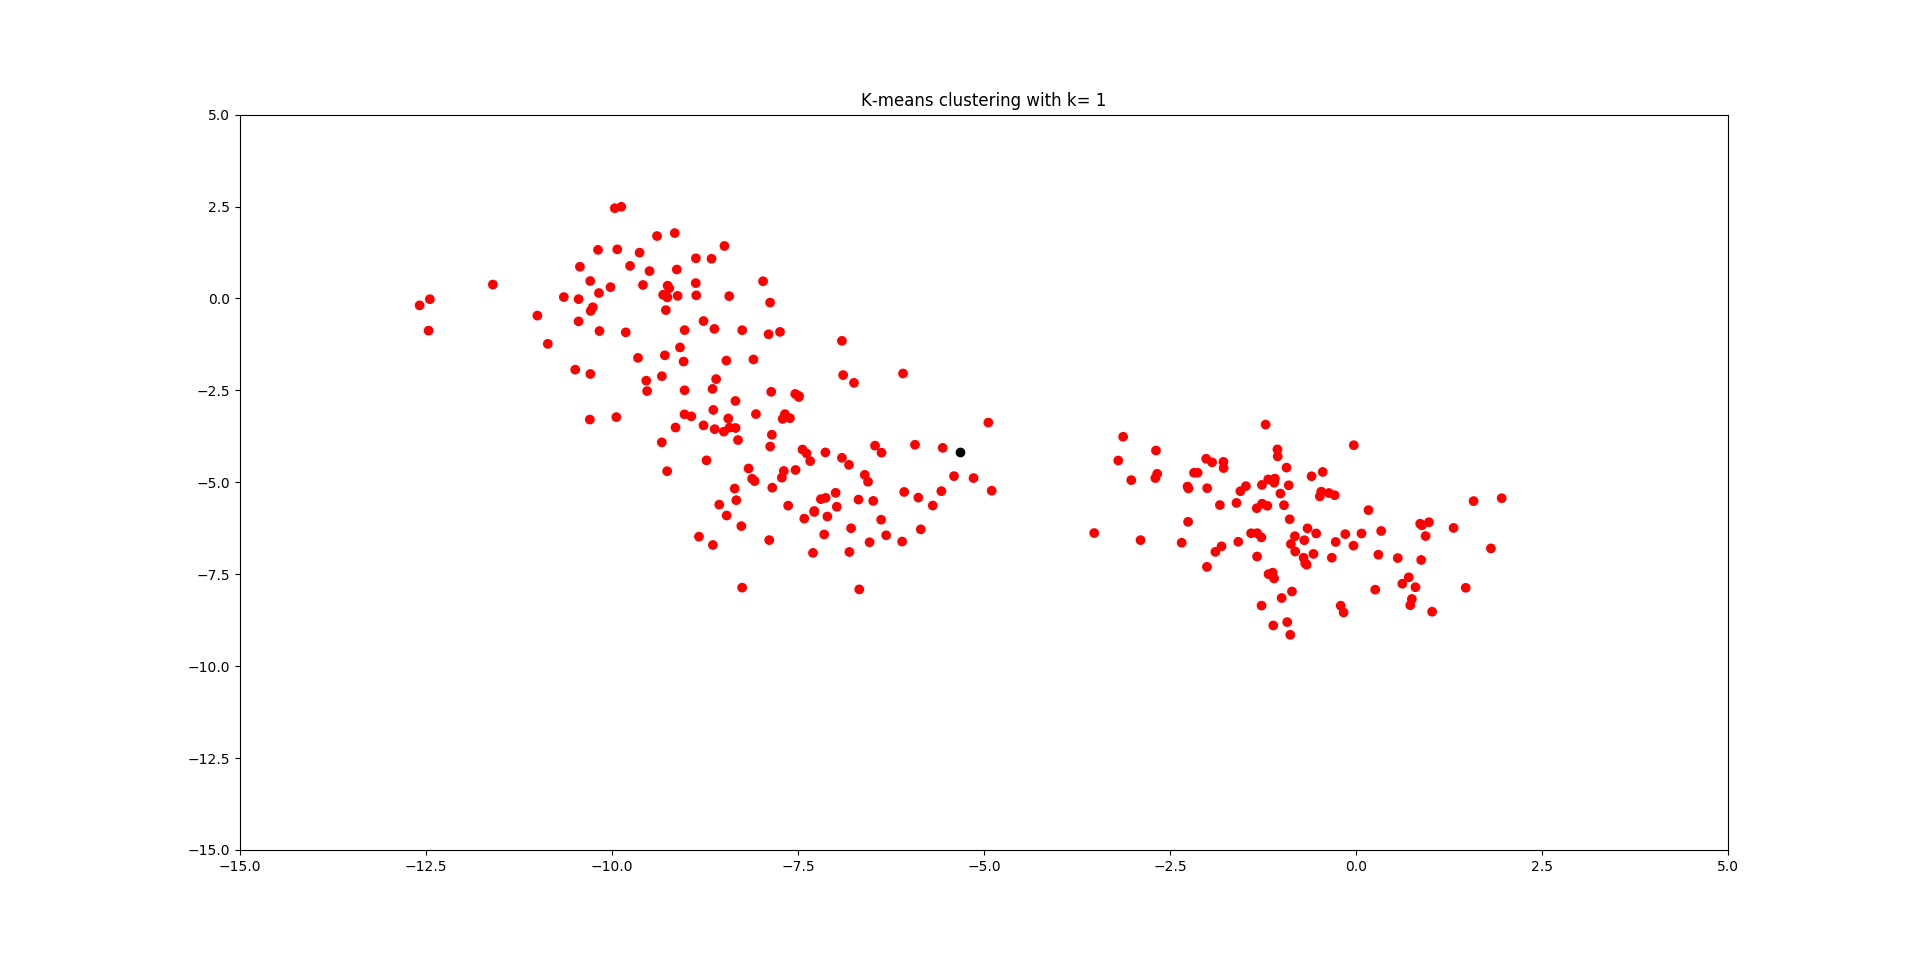
\includegraphics[scale=0.15]{11k1}
    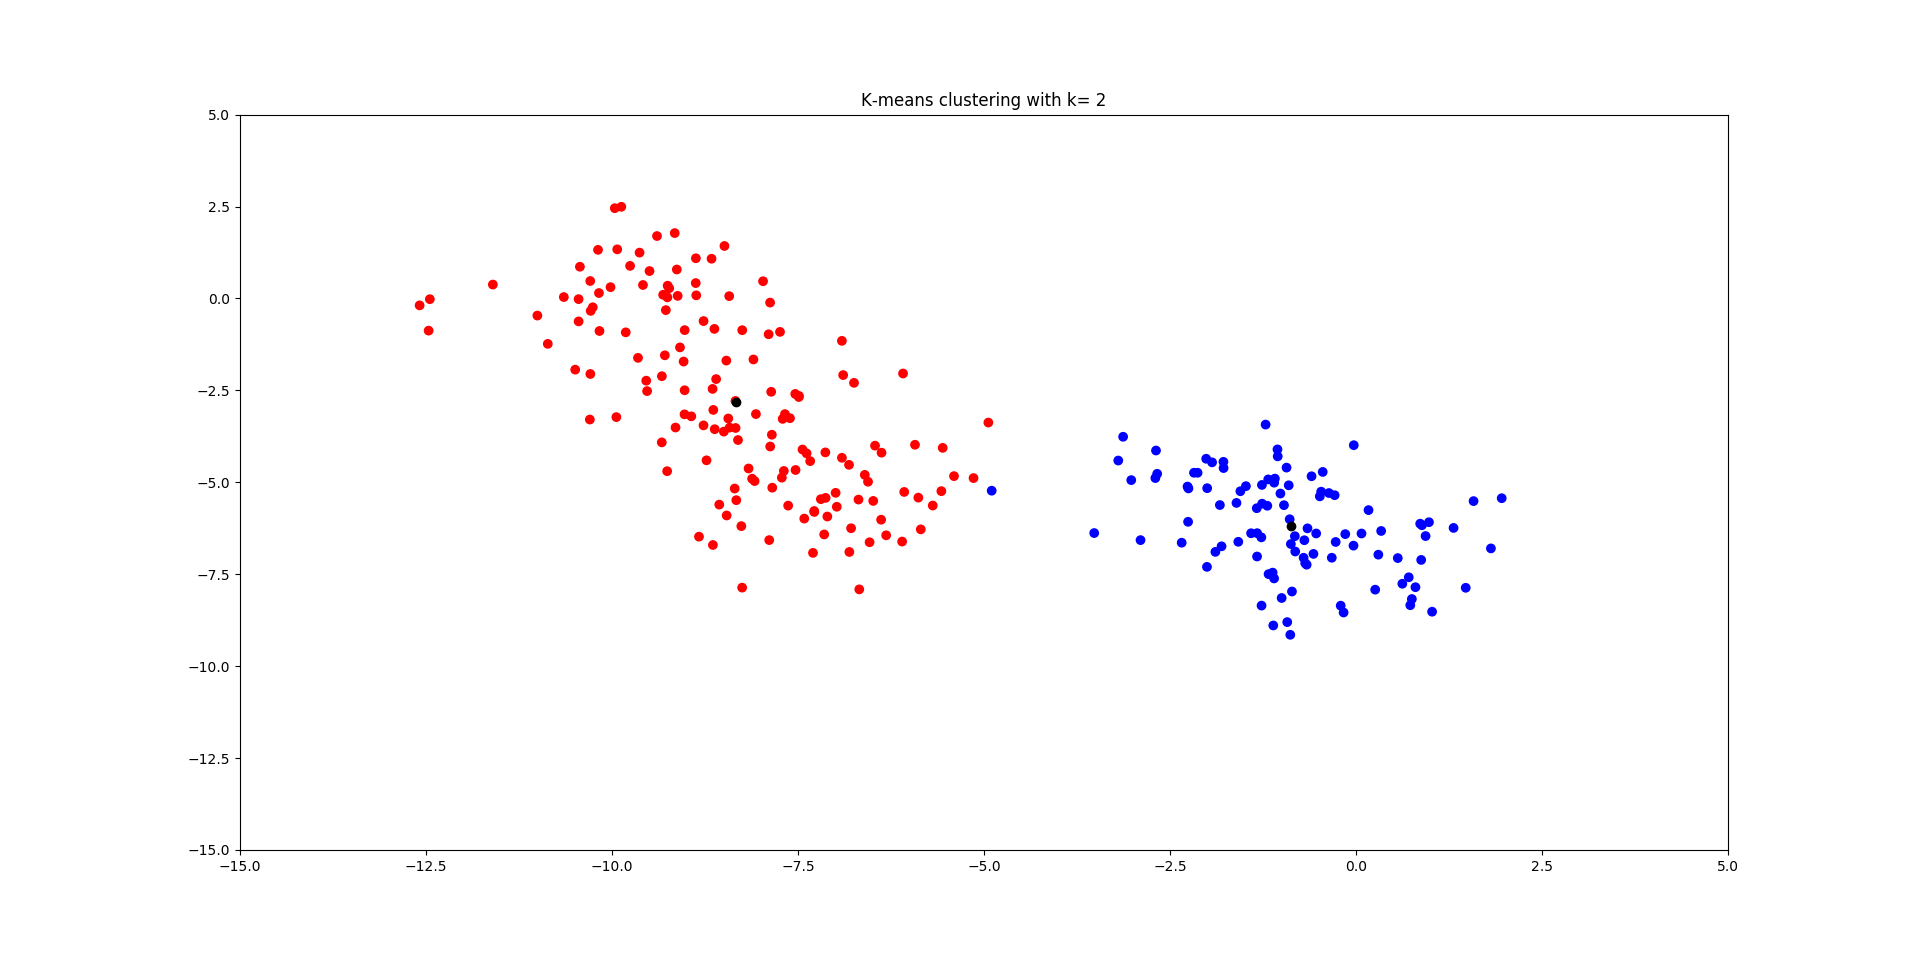
\includegraphics[scale=0.15]{11k2}
    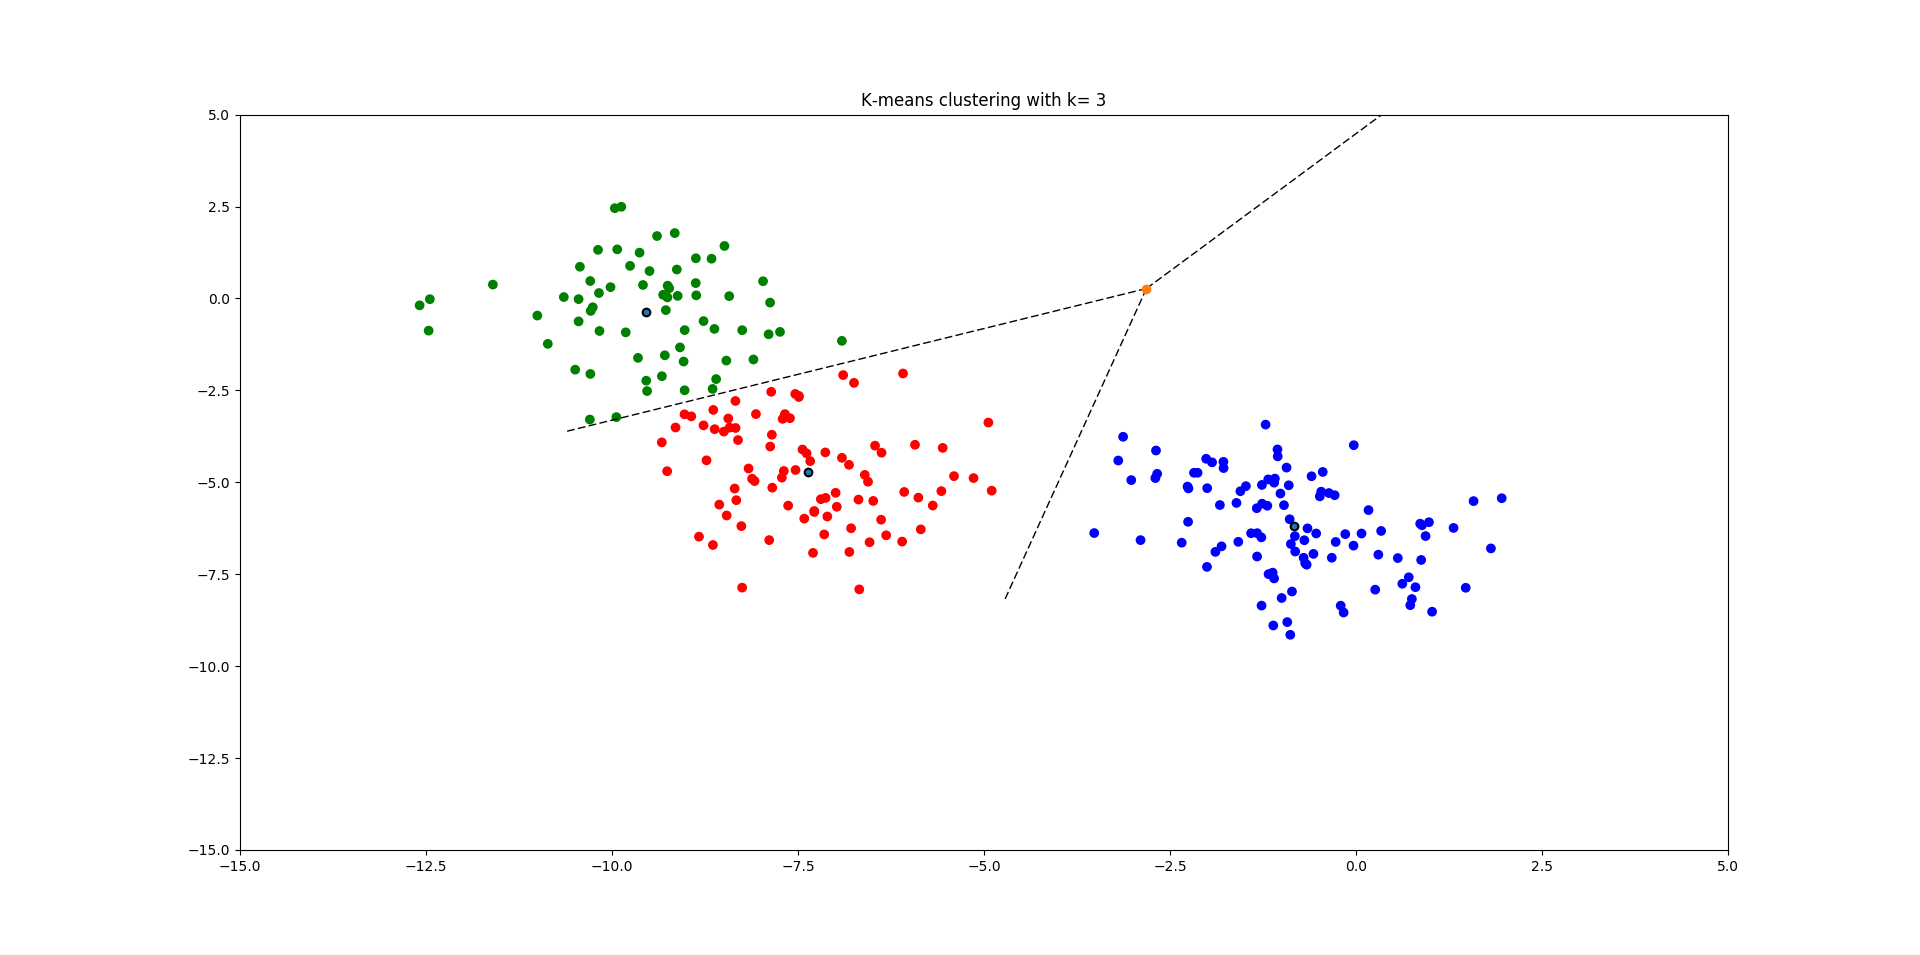
\includegraphics[scale=0.15]{11k3}
    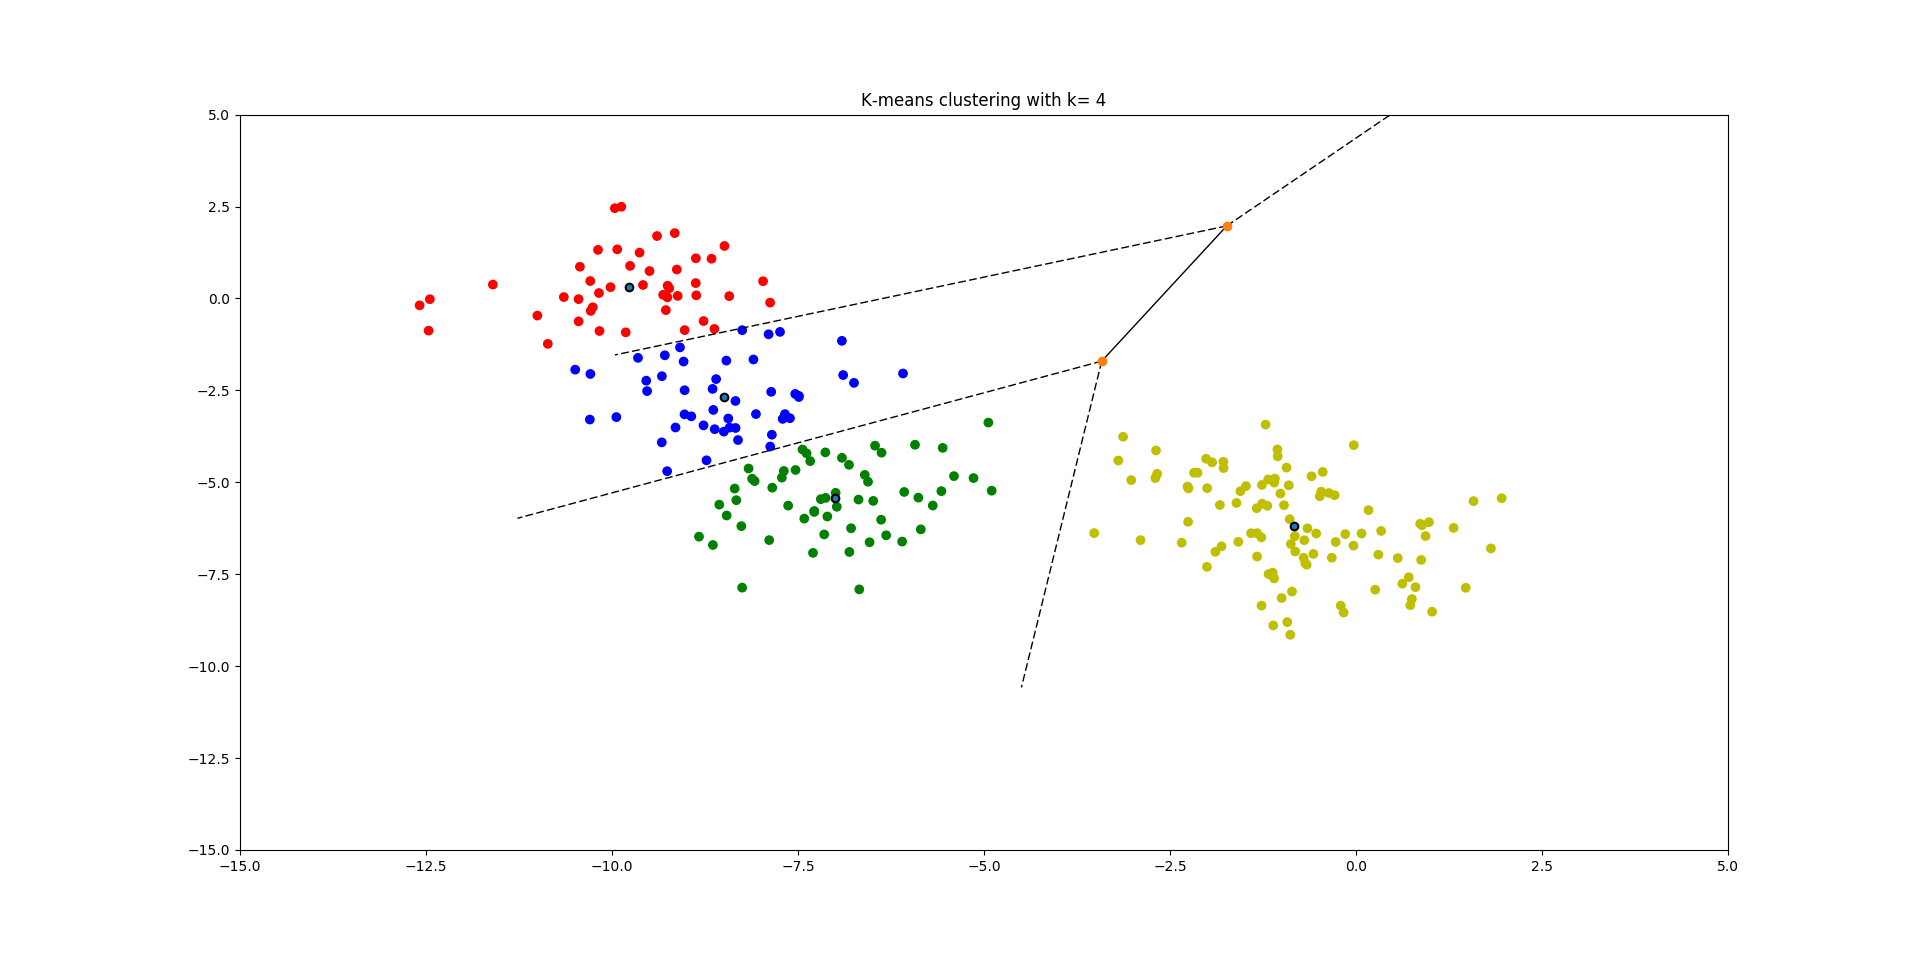
\includegraphics[scale=0.15]{11k4}
    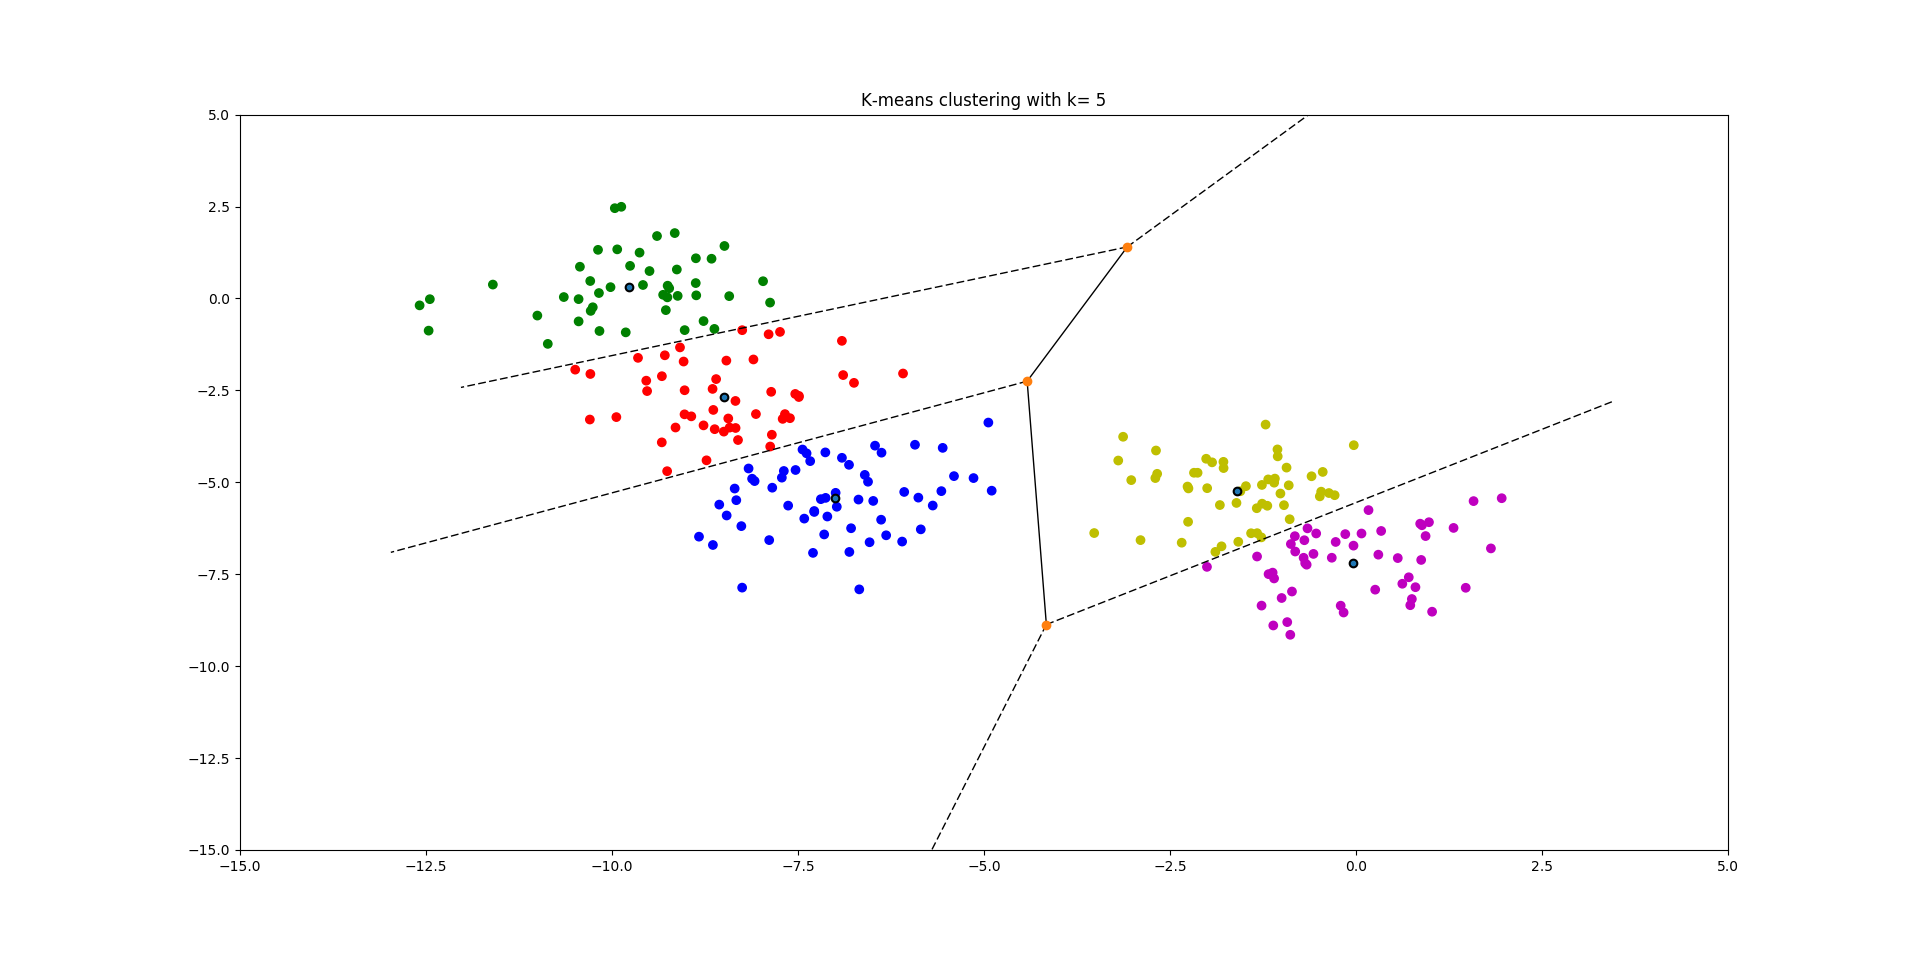
\includegraphics[scale=0.15]{11k5}
    \caption {plots for k=[1,2,3,4,5]}
\end{figure*}
\pagebreak

\section*{Question 4}
\vspace{3mm}
After running the EM algorithm for the Gaussian mixture model for cluster number of $K=[1,2,3,4,5]$, several times, I chose the plots for the following log-likelihood values: \\
\\
\begin{figure}[h]
    \centering  
    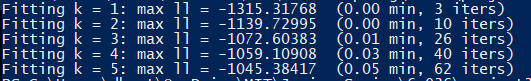
\includegraphics[scale=1.2]{14EMLL}
    \caption{log-likelihood values for EM algorithm}
\end{figure}
\\
\\


The plots I got are in the next page:


\begin{figure*}[h!]
    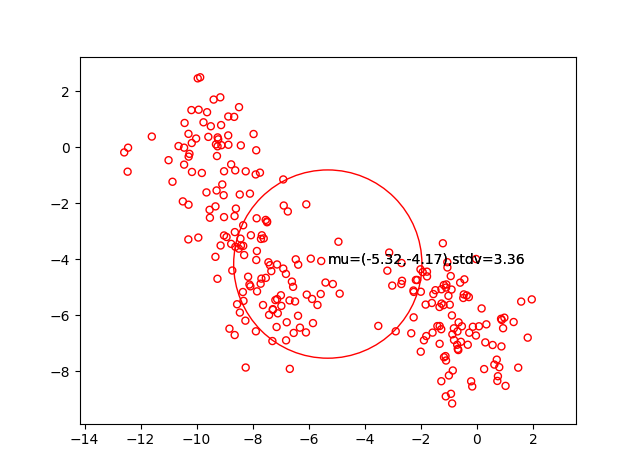
\includegraphics[scale=0.48]{14k1}
    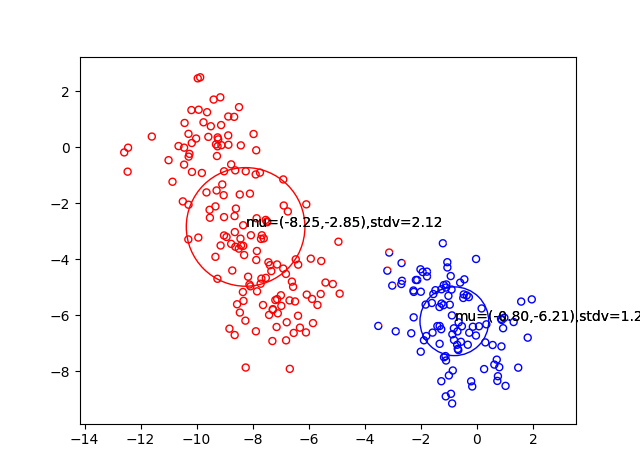
\includegraphics[scale=0.48]{14k2}
    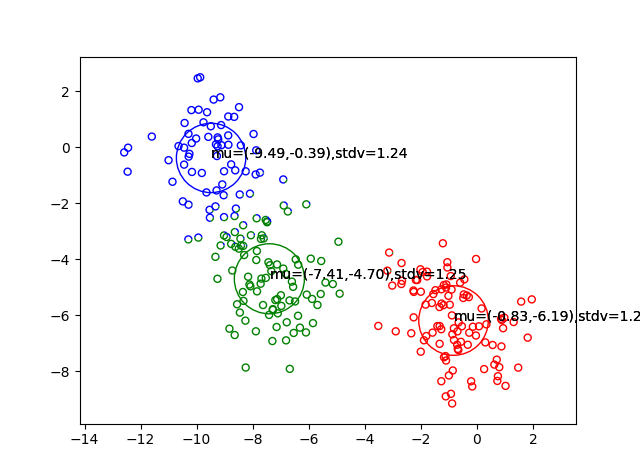
\includegraphics[scale=0.48]{14k3}
    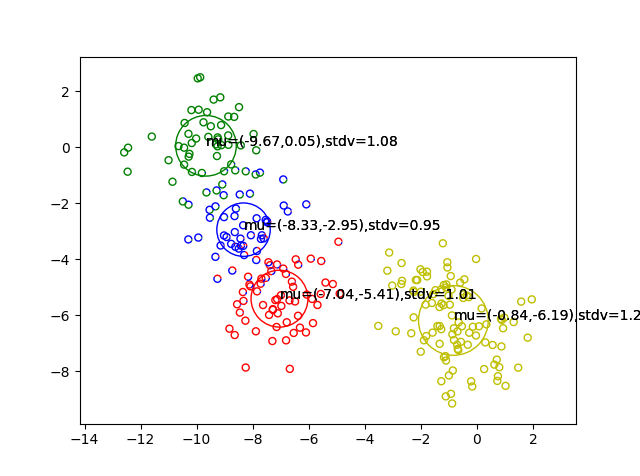
\includegraphics[scale=0.48]{14k4}
    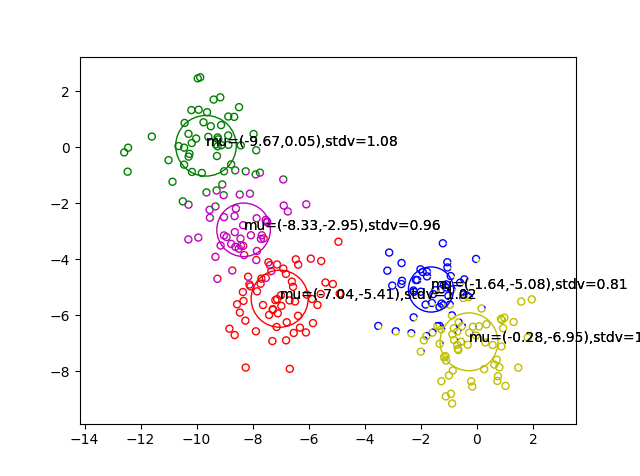
\includegraphics[scale=0.48]{14k5}
    \caption {plots for k=[1,2,3,4,5]}
\end{figure*}
\pagebreak
\section*{Question 4}


It is easily seen that the larger the K value, the more spread out the clusters will be and the smaller $\sigma^2$ will be. As we include more clusters, the algorithm sort the points into more specific groups instead of one larger and general one.


\pagebreak
\part*{Part II - Clustering Census Data}
\vspace{8mm}
\section{Question 1}
By assuming that the features are independent, we will have overconfident cluster assignments, as their distance will increase.  As the distance increases, so does the weight of the points that are far away. Since the weight of those points increases, the clusters will be more strictly separated.

\section{ E-Step}

From Bayes rule, we get that:
\begin{equation*}
    p(z^{(i)} \vert x^{(i)}, \pi, \alpha) = \frac{p(z^{(i)})p(x^{(i)} \vert z^{(i)}, \pi, \alpha)}{p(x^{(i)})}
\end{equation*}


By marginalizing over \(\pi,\alpha \), we get the following:

\begin{equation*}
    p(z^{(i)} \vert x^{(i)}, \pi, \alpha) = 
    \frac{\pi_k \cdot \prod_{d=1}^D \alpha_{k,d} [x_d^{(i)}]^{
    \ [\![ x_d^{(i)} \text{  is not missing}]\!]}} 
    {\sum_{j=1}^k\pi_j \cdot \prod_{d=1}^D\alpha_{j,d} [x_d^{(i)}]^{ 
    \ [\![ x_d^{(i)} \text{  is not missing}]\!]}}
\end{equation*}

\section{ M-Step}
% \setcounter{section}{3}
\subsection*{3.a) \ ML of $\pi$}
The maximum likelihood estimate of $\pi$ will be:

\begin{equation*}
    \pi_j = \frac
    {\sum_{i=1}^N p(z^{(i)=j} \vert x^{(i)}, \pi, \alpha )}
    {N}
\end{equation*}

\subsection*{3.b) \ ML of $\alpha$}

The maximum likelihood estimate of $\alpha$ will be:

\begin{equation*}
    \alpha_{k,d}[c] = \frac{1}{N} \cdot
    \sum^N_{i=1} p(z^{(i)}=j \vert x^{(i)}, \pi, \alpha) \cdot [\![x_d^{(i)} == c]\!]
\end{equation*}

\section*{Qiestion 5}
For different K values, the maximum Log Likelihood does not change much. This is expected since the algorithm should perform about the same for low numbers of cluster we need to classify such a large amount of points in.

\begin{figure}[h!]
    \centering
    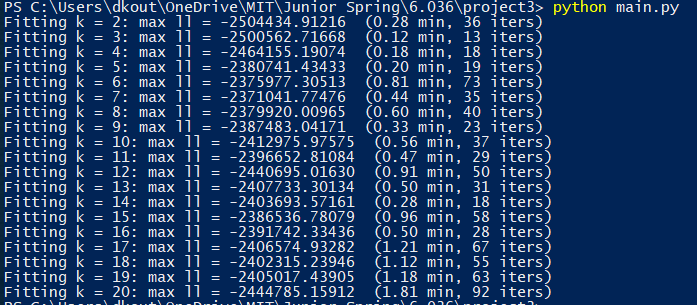
\includegraphics[scale=0.9]{25LL}
    \caption {Maximum Log Likelihood for different K values}
\end{figure}

However, when we see the trend of the log likelihood for only one k, we see that it increases significantly. For example, for k=4, we can see that the log-likelihood increases from $-499415$ to $2393848$. This can be seen in the following figure:

\begin{figure}[!ht]    
    \centering
    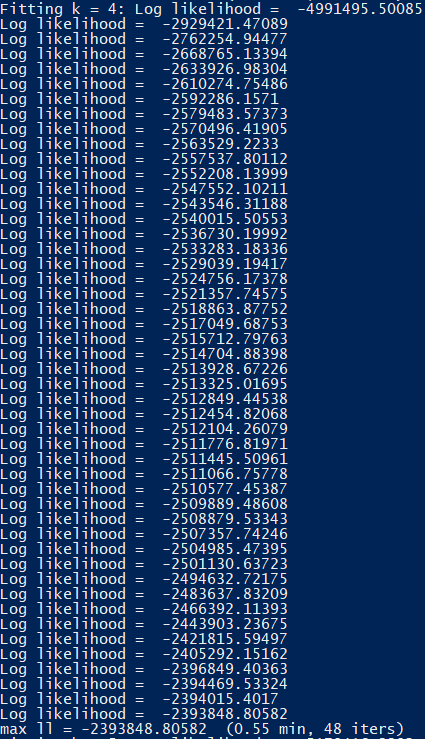
\includegraphics[scale=0.9]{25LL5}
    \caption {Log-Likelihood progression for k=4}
\end{figure}

\pagebreak

\clearpage

\newpage

\section*{Question 6}

Based on the figure shown below, the optimal value of $K$ is 7 when judging based on the Log-Likelihood (LL) as well as when judging based on the Bayesian Information Criterion (BIC). Both results agree.

\begin{figure}[!h]
    \centering
    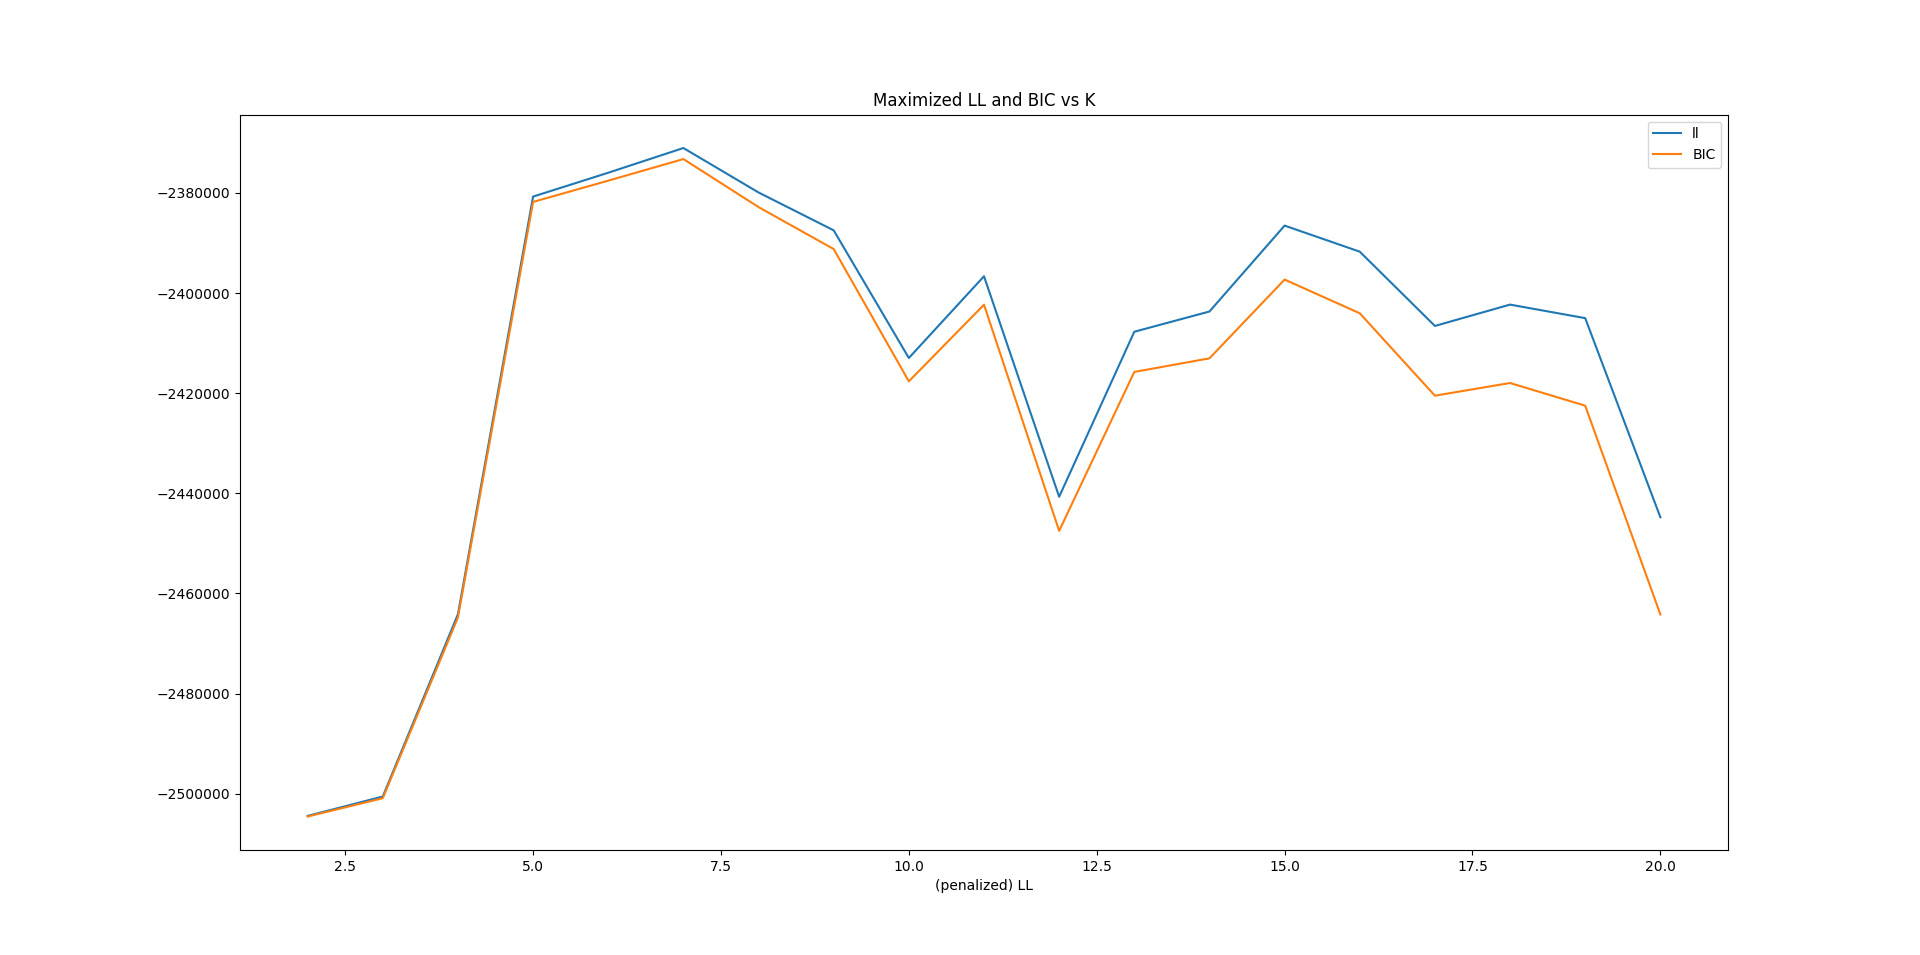
\includegraphics[scale=0.3]{BICvK}
    \caption{Graph of BIC and LL vs K}
\end{figure}
\pagebreak

\section*{Question 7}

\subsection*{(7.a)}
When calling \texttt{print\_clusters} with $K=7$, I get 7 clusters that are grouped by the following features:
\begin{itemize}
  \item age
  \item sex
  \item birthplace
  \item ancestry
  \item citizenship
  \item income
  \item education level
  \item employer
\end{itemize}

The clusters can be seen in the figure in the following page.
\\
If we run the model for a $K=10$, we can see that the clusters change a bit and become more specific. However, most of the clusters don't even change. The fact that many clusters stay the same, means that they are quite stable. One of the very few concepts added was "11th grade" for the educational level. It is clear that this is a bit too specific as can be easily inferred from the fact that we have more clusters. 

\begin{figure}[!ht]
    \centering
    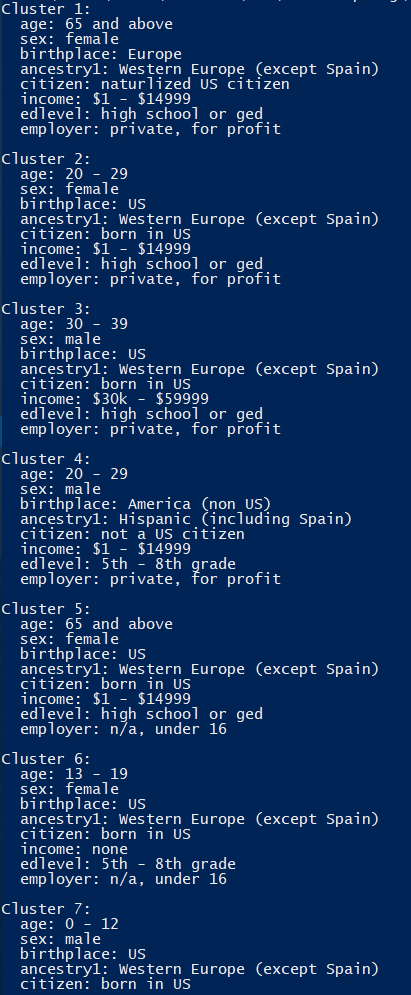
\includegraphics[scale=0.7]{clusters}
    \caption{example cluster}
\end{figure}
\pagebreak
\pagebreak

\subsection*{(7.b)}
 
 When running the model several times for $K=7$, we get a bit different clusters. More specific values such as age change quite a bit. However the clusters are not generally unstable. This change in the clusters (especially in age) is easily justifiable by the fact that there are more age groups than groups for other features.

\subsection*{(7.c)}
In order to judge how similar two states are, we can just train our model on two different states and make decisions based on the outputted features, number of clusters etc. By comparing how siimlar the features and the cluster separations are, we can gauge how similar the two states are. Two states that have the same clusters would be very similar, but two stats that have neither the same number of clusters nor the same cluster features would be very dissimilar.



\end{document}